\documentclass[8pt,a4paper]{beamer}

% PACKAGES
\usepackage[utf8]{inputenc}
\usepackage[T1]{fontenc}
\usepackage[francais]{babel}
%\usepackage{ucs} % Utilisation de l'unicode
%\usepackage{amsmath}
%\usepackage{amsfonts}
%\usepackage{amssymb}
\usepackage{graphicx}
\usepackage{fancybox}
%\usepackage{multimedia}
\usepackage{ragged2e} % Pour les textes justifiés
\usepackage{listings} % Intégration de listings de programmes
\usepackage{hyperref}

% CONFIGURATION DES PACKAGES
\hypersetup{
    bookmarks=true,         % show bookmarks bar?
    pdftoolbar=true,        % show Acrobat’s toolbar?
    pdfmenubar=true,        % show Acrobat’s menu?
    colorlinks=false,       % false: boxed links; true: colored links
    linkcolor=red,          % color of internal links
    citecolor=green,        % color of links to bibliography
    filecolor=magenta,      % color of file links
    urlcolor=cyan           % color of external links
}

% ragged2e
\justifying

% Listings
\lstset{ %
language=Python,                % the language of the code
basicstyle=\footnotesize,       % the size of the fonts that are used for the code
numbers=left,                   % where to put the line-numbers
numberstyle=\footnotesize,      % the size of the fonts that are used for the line-numbers
stepnumber=1,                   % the step between two line-numbers. If it's 1, each line 
                                % will be numbered
numbersep=5pt,                  % how far the line-numbers are from the code
backgroundcolor=\color{white},  % choose the background color. You must add \usepackage{color}
showspaces=false,               % show spaces adding particular underscores
showstringspaces=false,         % underline spaces within strings
showtabs=false,                 % show tabs within strings adding particular underscores
frame=single,                   % adds a frame around the code
tabsize=2,                      % sets default tabsize to 2 spaces
captionpos=b,                   % sets the caption-position to bottom
breaklines=true,                % sets automatic line breaking
breakatwhitespace=false,        % sets if automatic breaks should only happen at whitespace
keywordstyle=\color{red}\bfseries,  	% underlined bold black keywords
identifierstyle=,						% nothing happens
commentstyle=\color{gray}, 				% white comments
stringstyle=\ttfamily					% typewriter type for strings
}

% THEME

\usetheme{Frankfurt}
%\usetheme{Montpellier}
%\usetheme{Hannover}
%\usecolortheme{wolverine}
%\usetheme{Antibes}
%\usecolortheme{beaver}
%\usecolortheme{seahorse}
%\usecolortheme{dolphin}
%\useoutertheme{infolines}

% MODIFICATIONS DIVERSES
\setcounter{tocdepth}{1}
\setbeamertemplate{footline}[page number]
 %Gestion du numero de page
\setbeamertemplate{footline}
{%
\leavevmode%
\hbox{%
\begin{beamercolorbox}[wd=.5\paperwidth,ht=2.5ex,dp=1.125ex,right]{author
in head/foot}%
%\usebeamerfont{title in head/foot}\inserttitle\hspace{.3cm}
\usebeamerfont{title in head/foot}Outils numériques pour l'ingénieur\hspace{.3cm}
\end{beamercolorbox}%
\begin{beamercolorbox}[wd=.4\paperwidth,ht=2.5ex,dp=1.125ex,left]{title
in head/foot}%
\usebeamerfont{author in head/foot}\hspace{.3cm}\insertdate
\end{beamercolorbox}%
\begin{beamercolorbox}[wd=.1\paperwidth,ht=2.5ex,dp=1.125ex,center]{title
in head/foot}%
\usebeamerfont{author in
head/foot}\insertframenumber/\inserttotalframenumber
\end{beamercolorbox}%
}%
\vskip0pt%
}


%\renewcommand\Re{\operatorname{Re}}
%\renewcommand\Im{\operatorname{Im}}

\AtBeginSection[]
{
\begin{frame}{Plan}
\tableofcontents[currentsection]
\end{frame}
}
\graphicspath{{figures/}}


\author[LC]{\href{mailto:ludovic.charleux@univ-savoie.fr}{ludovic.charleux@univ-savoie.fr}}
\title{MGM657 Outils Numériques pour l'Ingénieur}
\subtitle{Optimisation}
%\subtitle{}
\date{}
\institute{\url{www.polytech.univ-savoie.fr}}


% DEBUT DU DOCUMENT
\begin{document}

% PAGE DE GARDE
\begin{frame}[plain]
%\begin{columns}[c]
%\column{.5\textwidth}
%\center{\includegraphics[width=.75\textwidth]{figures/logo_polytech.jpg}}
%\column{.5\textwidth}
%\center{\includegraphics[width=.75\textwidth]{figures/logo_univ-savoie.jpg}}
%\end{columns}
\titlepage
\tableofcontents
\end{frame}

\section{Introduction: courbe brachistochrone}

\begin{frame}{Courbe brachistochrone}
  \begin{columns}
  \column{.47\textwidth}  
  \begin{center}
  \input{figures/courbe_brachistochrone.pdf_tex} 
  \end{center}
  \column{.47\textwidth}  
  
  \begin{block}{Problème}
  \begin{itemize}
  \item On lâche une masse ponctuelle $M$ de masse $m$ en $A$ à $t=0 s$.
  \item Elle suit la trajectoire verte sans frottements.
  \item Elle arrive en $B$ en $t=t_f$.
  \item Quelle trajectoire minimise le temps de parcours $t_f$
  \end{itemize}
  \end{block}
  \end{columns}
\end{frame}

\begin{frame}{Courbe brachistochrone: problème simplifié}
  \begin{columns}
  \column{.47\textwidth}  
  \begin{center}
  \input{figures/courbe_brachistochrone_lin.pdf_tex} 
  \end{center}
  \column{.47\textwidth}  
  
  \begin{block}{Problème}
  \begin{itemize}
  \item Comment évolue l'accélération sur un segment ?
  \item Quel est le temps de parcours sur un segment ?
  \end{itemize}
  \end{block}
  \end{columns}
\end{frame}

\begin{frame}{Courbe brachistochrone: problème simplifié}
\lstinputlisting[firstline=26,lastline=44]{../Example_code/brachi1d.py}
\end{frame}

\begin{frame}{Courbe brachistochrone: problème simplifié à 1 n\oe ud}
  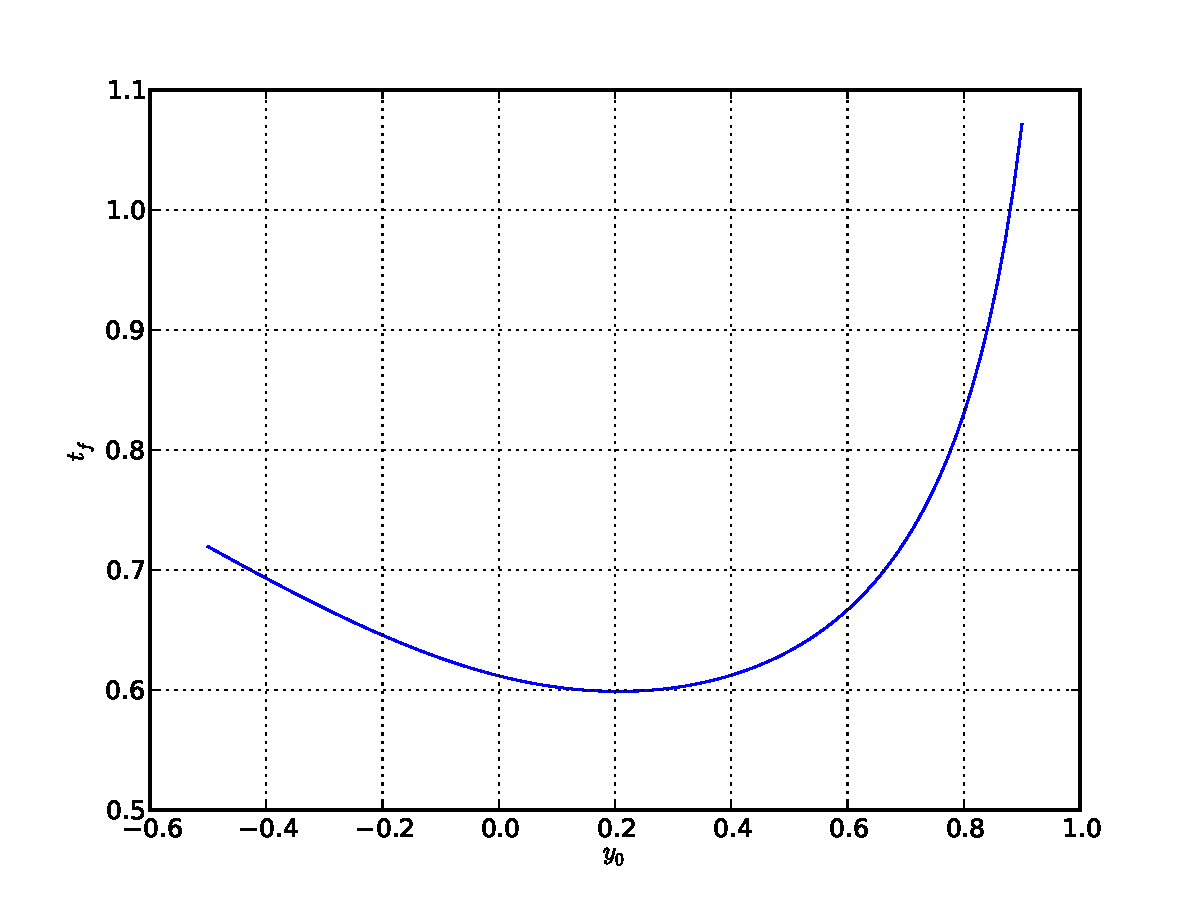
\includegraphics[width = 1\textwidth]{figures/brachi1d.pdf}
\end{frame}

\begin{frame}{Courbe brachistochrone: problème simplifié à 1 n\oe ud}
  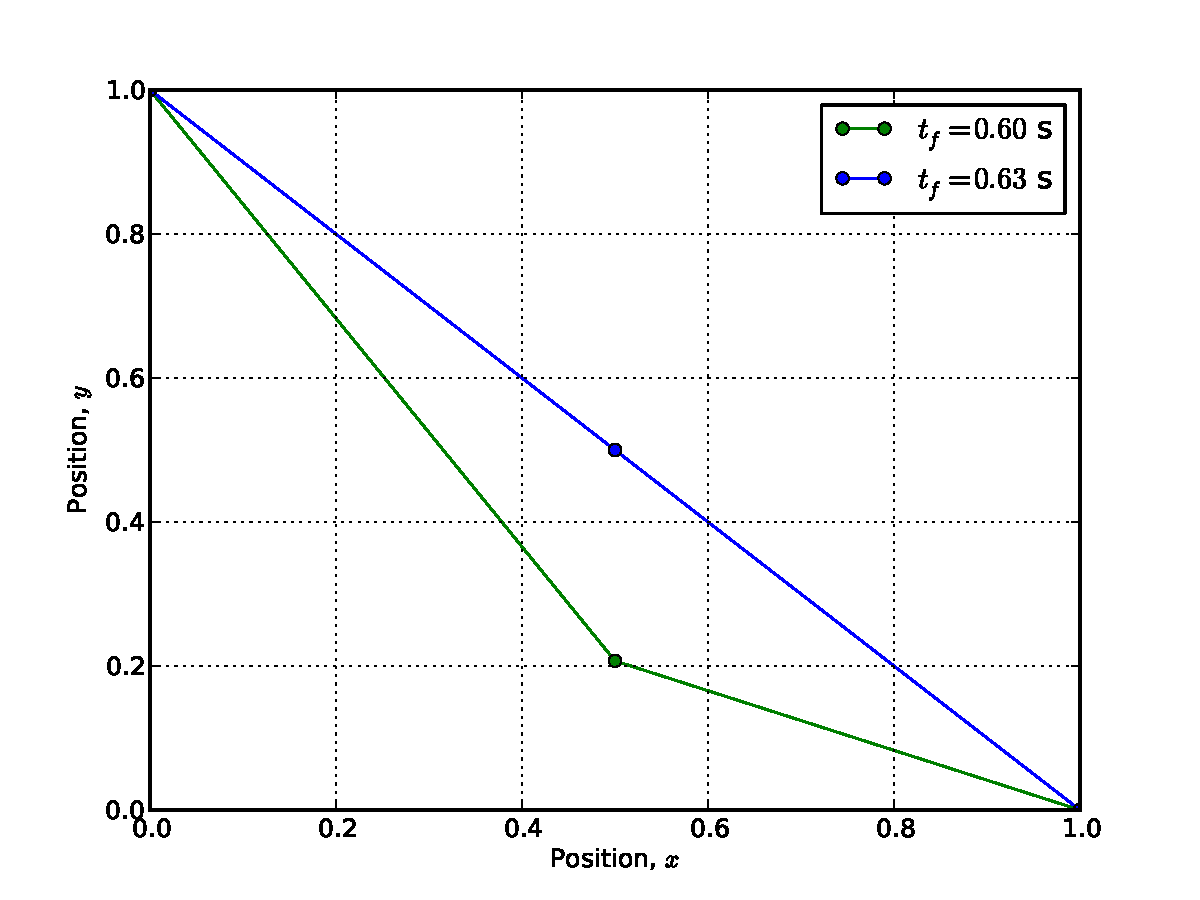
\includegraphics[width = 1\textwidth]{figures/brachi1d_sol.pdf}
\end{frame}

\begin{frame}{Courbe brachistochrone: problème simplifié à 2 n\oe ud}
  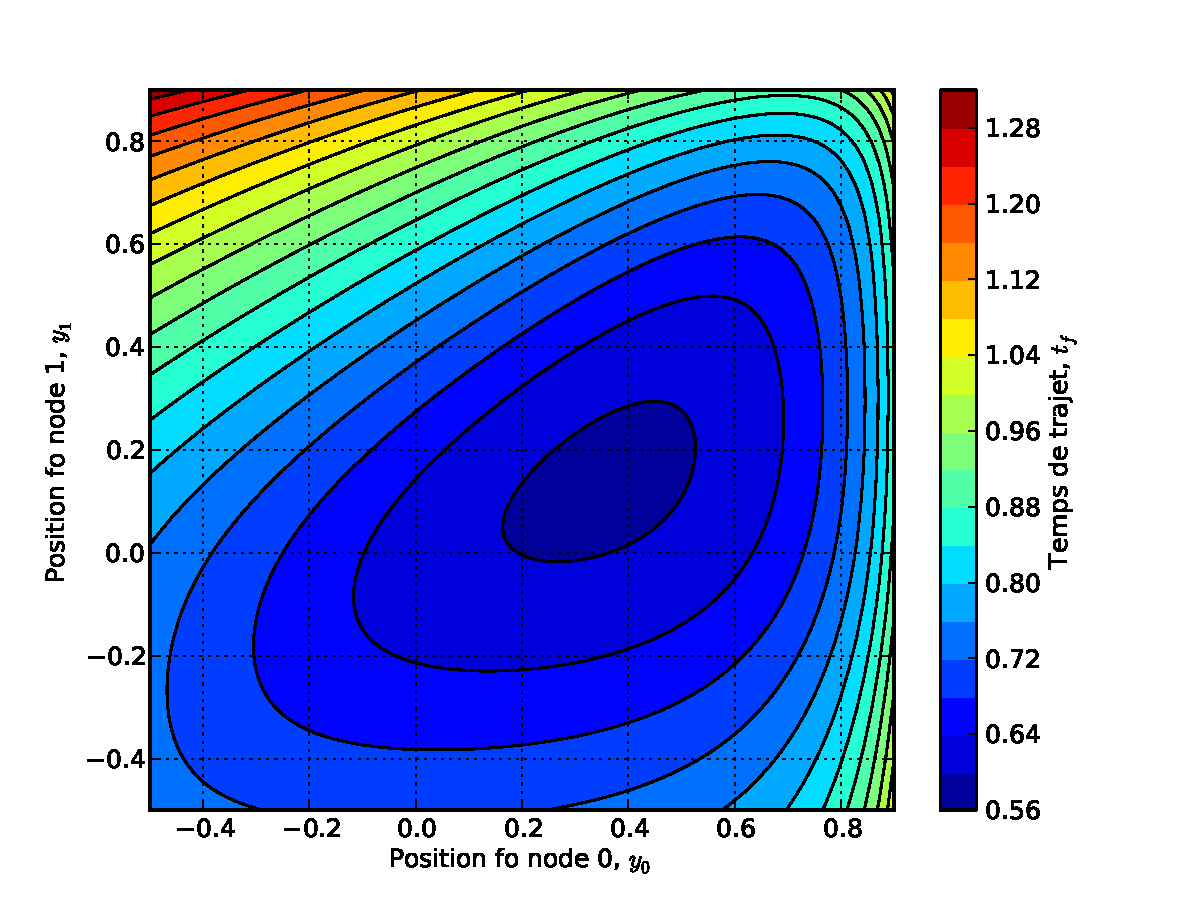
\includegraphics[width = 1\textwidth]{figures/brachi2d.pdf}
\end{frame}

\begin{frame}{Courbe brachistochrone: problème simplifié à 2 n\oe ud}
  \begin{center}
    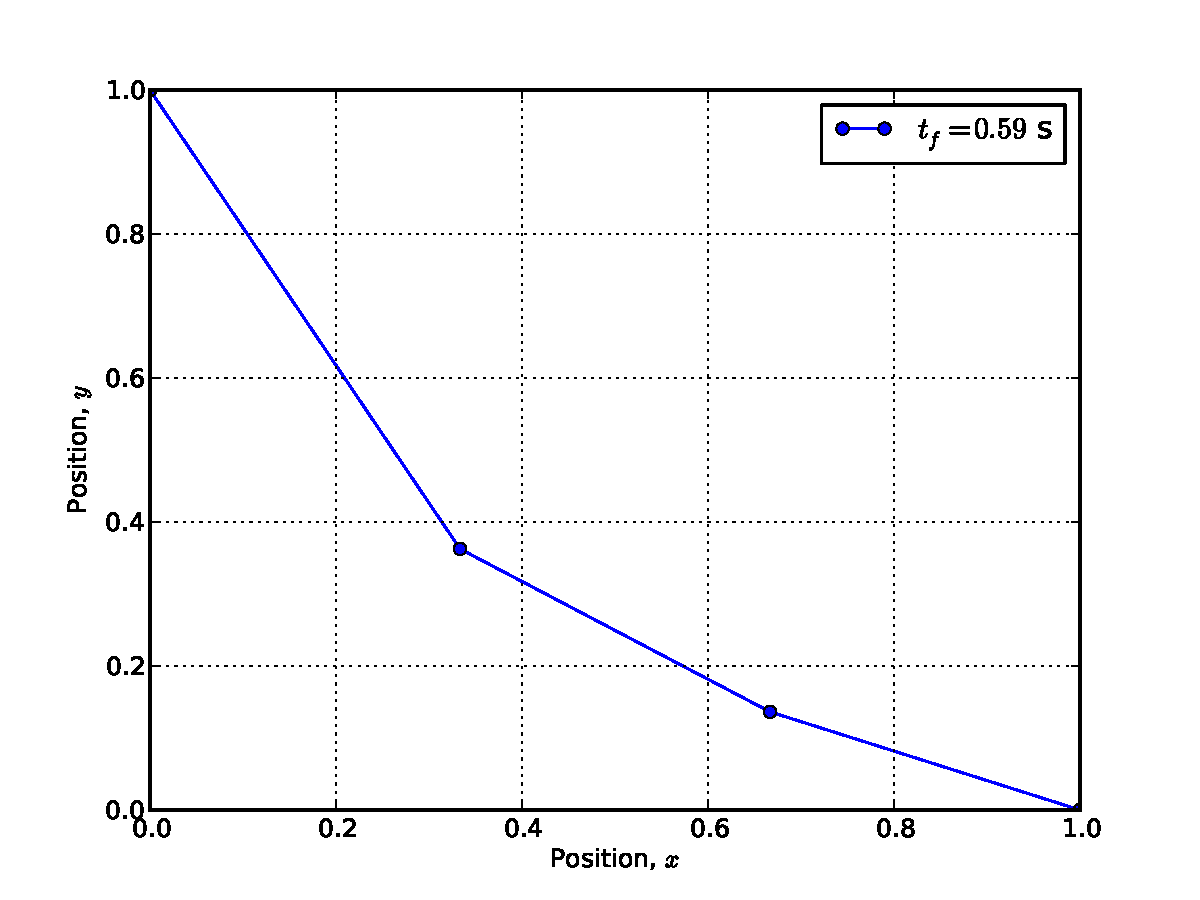
\includegraphics[width = 1.\textwidth]{figures/brachi2d_sol.pdf}
    
  \end{center}    


\end{frame}

\section{Formulation du problème général}

\begin{frame}{Formulation d'un problème d'optimisation}
    
  \begin{block}{Problème d'optimisation}
  \begin{itemize}
  \item Minimiser une fonctionnelle $f(X)$.
  \item La dimension $N$ du problème est celle de $X$. 
  \end{itemize}
  \end{block}
  
 \begin{block}{Approche pour résoudre}
  \begin{itemize}
  \item Évaluer $f$ le moins de fois possible.
  \item Trouver le minimum de $f$ et pas un minimum local.
  \end{itemize}
  \end{block} 
  
 \begin{block}{Champ d'application}
  \begin{itemize}
  \item Il est très vaste: mécanique, physique, économie, \ldots
  \item Sens de $f$: du temps, de l'énergie, de l'argent, \ldots
  \end{itemize}
  \end{block}   
  
\end{frame}

\section{Méthodes de résolution}

\begin{frame}{Force brute}
  
  \begin{center}
  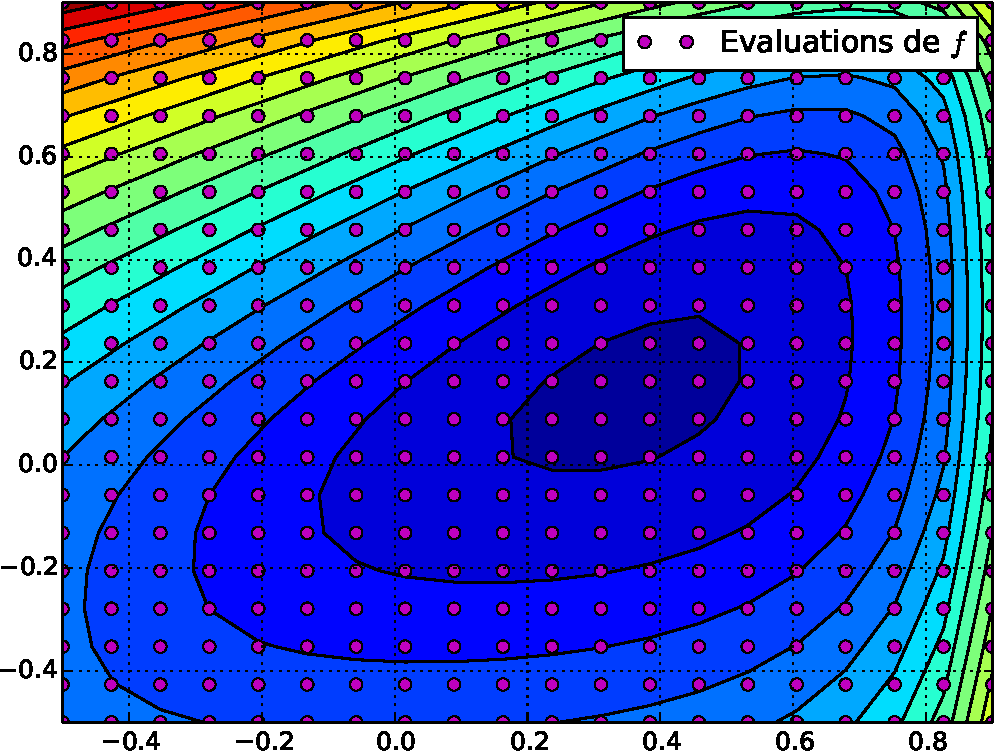
\includegraphics[width = .65\textwidth]{figures/brachi_BF.pdf}
  \end{center}
  
  
  \begin{block}{Fonctionnement}
  \begin{itemize}
  \item Discrétisation de chacune de composantes de $X$ en $P$ valeurs.
  \item Évaluation de $f$ en chaque point et recherche de la valeur minimale ($P^N$).
  \item Question: évaluer $f$ demande $1\mu$s. Avec $P=20$ et $N=100$, quel temps de calcul ?
  \end{itemize}
  \end{block}
 
\end{frame}




\begin{frame}{Simplexe / Nelder-Mead}
  
  \begin{center}
  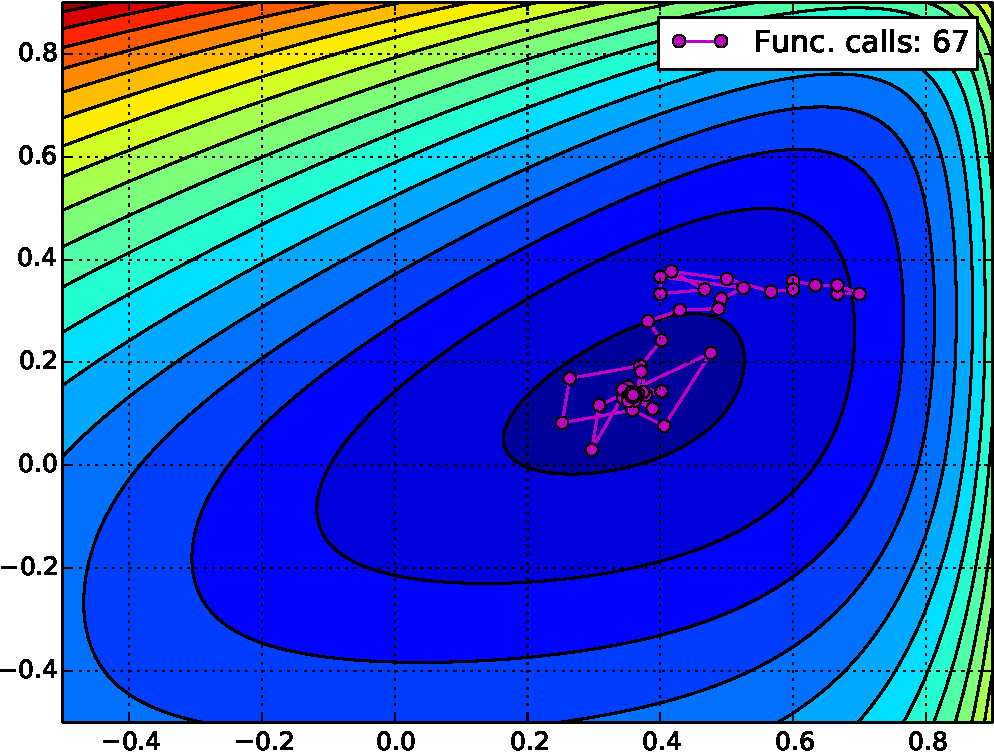
\includegraphics[width = .65\textwidth]{figures/brachi_NM.pdf}
  \end{center}
  
  
  \begin{block}{Fonctionnement}
  \begin{itemize}
  \item Construction d'un simplexe arbitraire (triangle en dimension 2).
  \item Déformation du simplexe pour converger vers la solution.
  \end{itemize}
  \end{block}
 
\end{frame}



\begin{frame}{Simplexe / Nelder-Mead: N = 10}
  
  \begin{center}
  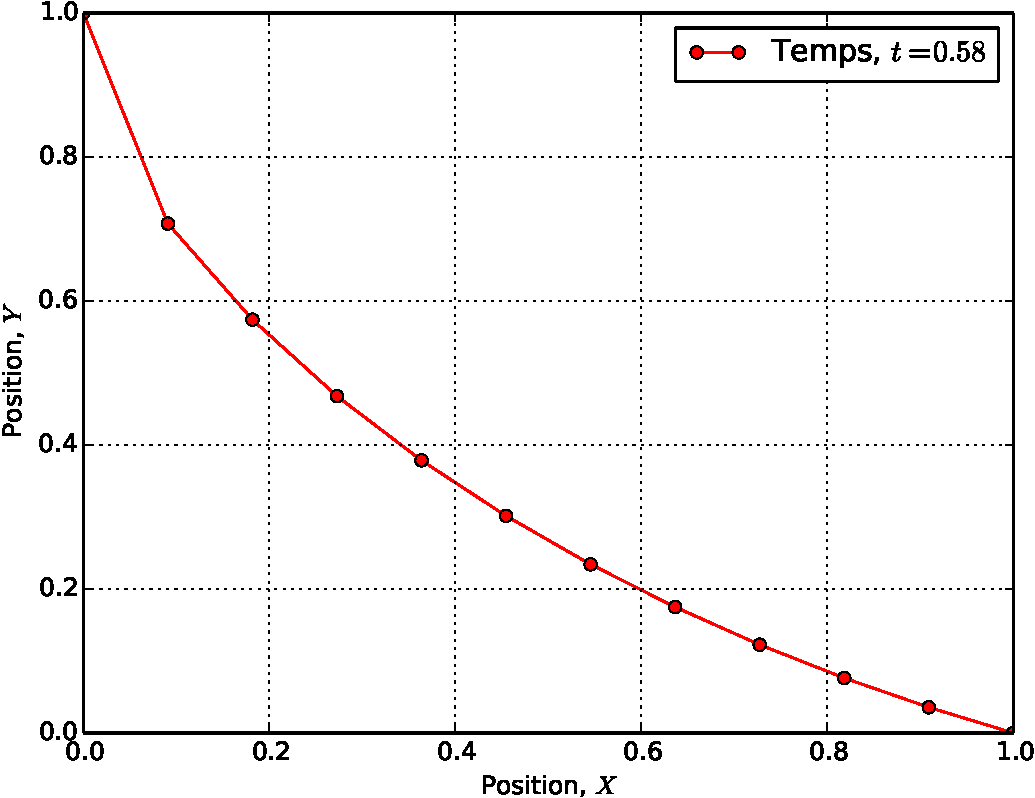
\includegraphics[width = .9\textwidth]{figures/brachi_NM_20D.pdf}
  \end{center}
\end{frame}

\begin{frame}{Algorithme de descente}
  
  \begin{block}{Fonctionnement}
  \begin{itemize}
  \item Calcul d'une direction de descente.
  \item Recherche linéaire dans cette direction.
  \item Exemple: algorithme du gradient, de Newton, BFGS, \ldots
  \end{itemize}
  \end{block}
 
\end{frame}

\section{Conclusions}
\begin{frame}{Conclusions}
  \begin{block}{Points positifs}
   \begin{itemize}
  \item Méthodes à très large spectre d'application.
  \item Il faut juste formuler la fonctionnelle $f$.
  \end{itemize}
  \end{block}
 \begin{alertblock}{Points négatifs}
   \begin{itemize}
  \item Évaluation de la qualité de la solution.
  \item Difficultés dans le cas de problèmes bruités.
  \item Conditionnement du problème parfois difficile.
  \end{itemize}
  \end{alertblock}
   
\end{frame}


\end{document}




